\scanpage{81}
On va graduer $K_{u,k}^{\bullet\bullet}$ par a) le degré extérieur venant de $\Lambda_k^*\Psi_k$ ($\deg_{\mathrm{ext}}\Gamma^i\otimes\Lambda^j=j$) et b) le \uline{degré total} $i+j$. Ainsi $d$ augmente le degré extérieur par $1$, et invarie le degré total \deleted{\unsure{Kde}} (le degré complémentaire est $\deg_{\mathrm{comp}}\Gamma^i\otimes\Lambda^j=i$, il est diminué de $1$ par $d$.) Muni du degré total (ou complémentaire) $K_{u\,k}^{\bullet\bullet}$ est une Algèbre graduée sur l'Anneau gradué $k\{T\}$.

Conséquence (de $\gamma$ \unsure{disons de suite})

\uline{Théorème} Soit $K^{\bullet\bullet}(X,u,k)=\Gamma(X,K_{u,k}^{\bullet\bullet})$.

Alors on a un hom can (du fait que $K_{u\,k}^{\bullet\bullet}$ \deleted{\unsure{$K$}} est une résolution de $k\{T\}$)
\[
\begin{aligned}
H^{**}\deleted{\unsure{K}}(X,u,k)&\overset{\mathrm{dfn}}{=}H^{**}(K^{\bullet\bullet}(X,u,k))\\
&\longrightarrow H^{**}(X,k\{T\})\\
&\simeq H^*(X,k)\otimes_{\mathbb Z}\mathbb Z\{T\}
\end{aligned}
\]
et ceci est un isomorphisme pour les bidegrés $(i,j)$ tels que $\deleted{\unsure{i\leq j}}j\leq i$, tandis que $H^{i,j}(X,u,k)=0$ (et pour cause) pour $j>i$.

\figure{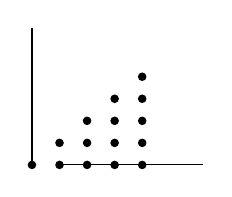
\begin{tikzpicture}[x=0.35cm,y=0.28cm]
\draw (0,6.2) -- (0,0); \draw (1,0) -- (6.2,0);
\foreach \x/\y in {0/0,1/0,1/1,2/0,2/1,2/2,3/0,3/1,3/2,3/3,4/0,4/1,4/2,4/3,4/4} {\fill (\x,\y) circle (1.55pt);}
\end{tikzpicture}}

\uline{Corollaire plus général.} Soit $f:X\unsure{\mathord{-}|\to}Y$ un morphisme de topos. Alors
\[
f_*K_{u,k}^{\bullet\bullet}\longrightarrow\mathbb R f_*(k\{T\})\simeq\mathbb R f_*(k)\otimes_{\mathbb Z}\mathbb Z\{\unsure{R|T}\}
\]
% archive sheet number: 80
